% Options for packages loaded elsewhere
\PassOptionsToPackage{unicode}{hyperref}
\PassOptionsToPackage{hyphens}{url}
%
\documentclass[
]{article}
\usepackage{amsmath,amssymb}
\usepackage{iftex}
\ifPDFTeX
  \usepackage[T1]{fontenc}
  \usepackage[utf8]{inputenc}
  \usepackage{textcomp} % provide euro and other symbols
\else % if luatex or xetex
  \usepackage{unicode-math} % this also loads fontspec
  \defaultfontfeatures{Scale=MatchLowercase}
  \defaultfontfeatures[\rmfamily]{Ligatures=TeX,Scale=1}
\fi
\usepackage{lmodern}
\ifPDFTeX\else
  % xetex/luatex font selection
\fi
% Use upquote if available, for straight quotes in verbatim environments
\IfFileExists{upquote.sty}{\usepackage{upquote}}{}
\IfFileExists{microtype.sty}{% use microtype if available
  \usepackage[]{microtype}
  \UseMicrotypeSet[protrusion]{basicmath} % disable protrusion for tt fonts
}{}
\makeatletter
\@ifundefined{KOMAClassName}{% if non-KOMA class
  \IfFileExists{parskip.sty}{%
    \usepackage{parskip}
  }{% else
    \setlength{\parindent}{0pt}
    \setlength{\parskip}{6pt plus 2pt minus 1pt}}
}{% if KOMA class
  \KOMAoptions{parskip=half}}
\makeatother
\usepackage{xcolor}
\usepackage[margin=1in]{geometry}
\usepackage{graphicx}
\makeatletter
\def\maxwidth{\ifdim\Gin@nat@width>\linewidth\linewidth\else\Gin@nat@width\fi}
\def\maxheight{\ifdim\Gin@nat@height>\textheight\textheight\else\Gin@nat@height\fi}
\makeatother
% Scale images if necessary, so that they will not overflow the page
% margins by default, and it is still possible to overwrite the defaults
% using explicit options in \includegraphics[width, height, ...]{}
\setkeys{Gin}{width=\maxwidth,height=\maxheight,keepaspectratio}
% Set default figure placement to htbp
\makeatletter
\def\fps@figure{htbp}
\makeatother
\setlength{\emergencystretch}{3em} % prevent overfull lines
\providecommand{\tightlist}{%
  \setlength{\itemsep}{0pt}\setlength{\parskip}{0pt}}
\setcounter{secnumdepth}{-\maxdimen} % remove section numbering
\usepackage{amsmath}
\renewcommand{\familydefault}{\sfdefault}
\usepackage[colorlinks=true, citecolor=blue, urlcolor=blue,linkcolor=blue, pdfborder={0 0 0}]{hyperref}
\urlstyle{same}
\usepackage{xcolor}
\usepackage{booktabs}
\raggedright
\usepackage{listings}
\ifLuaTeX
  \usepackage{selnolig}  % disable illegal ligatures
\fi
\usepackage{bookmark}
\IfFileExists{xurl.sty}{\usepackage{xurl}}{} % add URL line breaks if available
\urlstyle{same}
\hypersetup{
  pdftitle={Evaluating an attempt to restore summer fire in the Northern Great Plains},
  pdfauthor={Devan Allen McGranahan and Jay P. Angerer},
  hidelinks,
  pdfcreator={LaTeX via pandoc}}

\title{Evaluating an attempt to restore summer fire in the Northern
Great Plains}
\usepackage{etoolbox}
\makeatletter
\providecommand{\subtitle}[1]{% add subtitle to \maketitle
  \apptocmd{\@title}{\par {\large #1 \par}}{}{}
}
\makeatother
\subtitle{Supplementary Information}
\author{Devan Allen McGranahan and Jay P. Angerer}
\date{}

\begin{document}
\maketitle

\section{Additional data and results}\label{additional-data-and-results}

\subsection{Seasonal trends}\label{seasonal-trends}

\begin{figure}
\centering
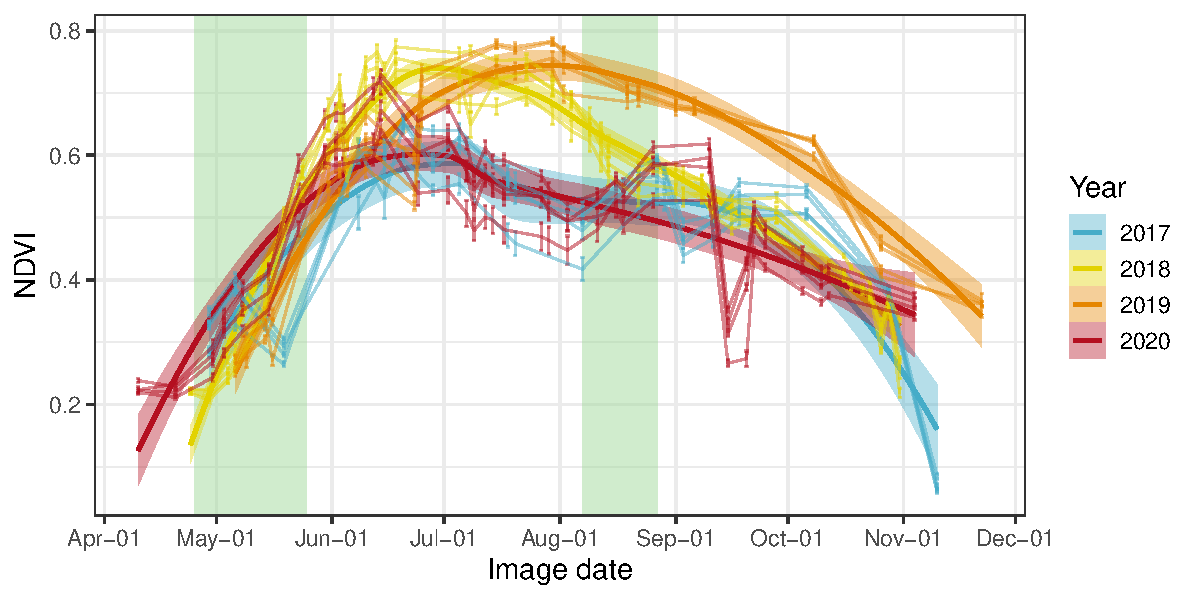
\includegraphics{SupplementalInformation_files/figure-latex/ndvi_trend-1.pdf}
\caption{Seasonal trends in Landsat-derived NDVI for the study period.
Green shaded areas span the first and last dates of completed burns in
the spring and summer.}
\end{figure}

\begin{figure}
\centering
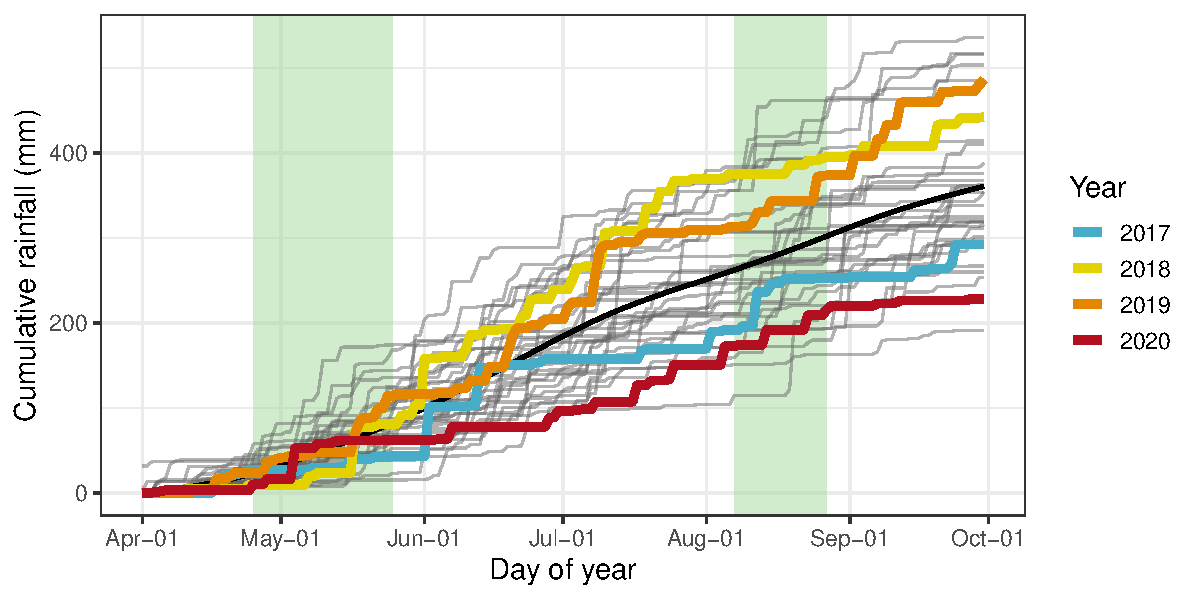
\includegraphics{SupplementalInformation_files/figure-latex/precip_trend-1.pdf}
\caption{Historical precipitation data for the entire 42-year period.
Thick black line shows smoothed 42-yr trend, gray lines individual
years, and colored lines study years. Green shaded areas span the first
and last dates of completed burns in the spring and summer.}
\end{figure}

\clearpage

\subsection{\texorpdfstring{\(z\) scores for historical data by burn
season}{z scores for historical data by burn season}}\label{z-scores-for-historical-data-by-burn-season}

\begin{table}[ht]
\centering
\begin{tabular}{llllll}
  \hline
Variable & Year & Spring 1990-99 & Spring 2012-22 & Summer 1990-99 & Summer 2012-22 \\ 
  \hline
Fuelbed Greenness (NDVI) & 2017 & Above (1.3) & Within (0.96) & Within (0.34) & Within (-0.05) \\ 
    & 2018 & Within (0.15) & Within (-0.87) & Within (0.92) & Within (0.64) \\ 
    & 2019 & Within (-0.54) & Below (-1.96) & Above (1.67) & Above (1.51) \\ 
    & 2020 & Above (1) & Within (0.48) & Within (0.37) & Within (-0.01) \\ 
  Cumulative rainfall & 2017 & Within (-0.63) & Within (-0.89) & Within (-0.89) & Within (-0.91) \\ 
    & 2018 & Within (-0.76) & Below (-1.08) & Above (1.87) & Above (1.38) \\ 
    & 2019 & Within (-0.27) & Within (-0.37) & Above (1.04) & Within (0.69) \\ 
    & 2020 & Within (0.02) & Within (0.06) & Below (-1.16) & Below (-1.13) \\ 
  Dew Point & 2017 & Below (-1.21) & Within (-0.98) & Below (-1.15) & Below (-1.07) \\ 
    & 2018 & Within (-0.05) & Within (0.63) & Within (-0.27) & Within (-0.07) \\ 
    & 2019 & Below (-1.01) & Within (-0.7) & Within (-0.21) & Within (0) \\ 
    & 2020 & Within (0.41) & Above (1.28) & Within (0.9) & Above (1.27) \\ 
  Relative Humidity & 2017 & Within (-0.85) & Within (-0.46) & Within (-0.56) & Within (-0.37) \\ 
    & 2018 & Within (-0.99) & Within (-0.67) & Within (-0.82) & Within (-0.65) \\ 
    & 2019 & Within (-0.48) & Within (0.12) & Within (0.67) & Above (1.01) \\ 
    & 2020 & Within (0.37) & Above (1.43) & Within (0.32) & Within (0.62) \\ 
  Vapor Pressure Deficit & 2017 & Within (0.48) & Within (0.26) & Within (-0.17) & Within (-0.32) \\ 
    & 2018 & Above (1.26) & Above (1.3) & Within (0.91) & Within (0.82) \\ 
    & 2019 & Within (-0.38) & Within (-0.9) & Below (-1.15) & Below (-1.36) \\ 
    & 2020 & Within (-0.62) & Below (-1.21) & Within (-0.13) & Within (-0.28) \\ 
  Wind speed & 2017 & Within (-0.69) & Within (-0.19) & Below (-1.69) & Within (-0.91) \\ 
    & 2018 & Within (-0.97) & Within (-0.42) & Below (-2.06) & Below (-1.31) \\ 
    & 2019 & Below (-1.54) & Within (-0.89) & Below (-1.3) & Within (-0.5) \\ 
    & 2020 & Below (-1.24) & Within (-0.65) & Within (-0.74) & Within (0.1) \\ 
   \hline
\end{tabular}
\caption{Seasonal deviations in fuel conditions and fire weather for spring and summer burn seasons, relative to two decades (1990-1999, 2012-2022) as presented in Fig. 4. Anomalies determined by $z$ scores (parentheses) and categorized as above, below, or within 1 standard deviation of the mean for the given historical range. 2018 and 2019 were the years in which no summer burns were conducted; all spring burns were conducted in all years} 
\end{table}

\newpage

\section{Script}\label{script}

This document provides script for fetching remotely-sensed imagery and
processing results in the \textsf{R} statistical environment.

\subsection{Remote sensing}\label{remote-sensing}

\subsubsection{Sentinel-2}\label{sentinel-2}

This \texttt{EvalScript} can be used in the
\href{https://browser.dataspace.copernicus.eu/}{Copernicus browser} as a
Custom script to create a Custom visualization that can be exported as a
16-bit \texttt{.tiff} for raster analysis. The user must select the area
of interest and imagery dates and is responsible for assessing
cloudiness.

\begin{lstlisting}[language=Java]

//VERSION=3
function setup() {
  return {
    input: ["B04", "B08", "B8A", "B11", "B12"],
    output: { bands: 2, sampleType: "UINT16" }
  };
}

function evaluatePixel(sample) {
  let nbr = index(sample.B08, sample.B12);
  let ndvi = index(sample.B08, sample.B04);
  // apply offset for UINT16 
  return [10000 * nbr + 10000, 
          10000 * ndvi + 10000]; 
}
\end{lstlisting}

\clearpage

\subsubsection{Landsat}\label{landsat}

This script for \href{https://code.earthengine.google.com/}{Google Earth
Engine} exports a composited NDVI \texttt{.tiff} file to the user's
Google Drive for the area of interest defined as \texttt{geometry} for
an eight week period beginning with each date given in
\texttt{listDate}. The script combines imagery from Landsat missions 5,
7, \& 8 and handles cloud masking.

\begin{lstlisting}[language=Java]
// Geometry
var geometry: Polygon, 4 vertices
  type: Polygon
  coordinates: List (1 element)
    0: List (5 elements)
      0: [-99.51276195869765,46.71741699210676]
      1: [-99.42521465645156,46.71741699210676]
      2: [-99.42521465645156,46.778346255312734]
      3: [-99.51276195869765,46.778346255312734]
      4: [-99.51276195869765,46.71741699210676]
  geodesic: false

// Main script

var batch = require('users/fitoprincipe/geetools:batch');

///****variables that need to be changed by user
//****ADD google drive directory name that you want to download files to
var gdrivedir = 'landsat'

var listDate= ["1992-04-20", "1992-07-20", "1993-04-20", "1993-07-20", 
               "1994-04-20", "1994-07-20", "1995-04-20", "1995-07-20", 
               "1996-04-20", "1996-07-20", "1997-04-20", "1997-07-20", 
               "1998-04-20", "1998-07-20", "1999-04-20", "1999-07-20", 
               "2000-04-20", "2000-07-20", "2001-04-20", "2001-07-20", 
               "2002-04-20", "2002-07-20", "2003-04-20", "2003-07-20",
               "2004-04-20", "2004-07-20", "2005-04-20", "2005-07-20", 
               "2006-04-20", "2006-07-20", "2007-04-20", "2007-07-20", 
               "2008-04-20", "2008-07-20", "2009-04-20", "2009-07-20",
               "2010-04-20", "2010-07-20", "2011-04-20", "2011-07-20", 
               "2012-04-20", "2012-07-20", "2013-04-20", "2013-07-20", 
               "2014-04-20", "2014-07-20", "2015-04-20", "2015-07-20",
               "2016-04-20", "2016-07-20", "2017-04-20", "2017-07-20", 
               "2018-04-20", "2018-07-20", "2019-04-20", "2019-07-20", 
               "2020-04-20", "2020-07-20", "2021-04-20", "2021-07-20",
               "2022-04-20", "2022-07-20"]

listDate.forEach(function (listDate) {
  //yearRanges.forEach(function (yearRange) {
    exportTimeseries(listDate)
  })
//})
function exportTimeseries(listDate) {
  
  // Defines a base date/time for the following examples.
  var startDate = ee.Date(listDate);
  print(startDate, 'The start date/time');
  print(startDate.format('YYYYMMdd'))
  var sdate = startDate.format('YYYYMMdd')
  var endDate = startDate.advance(8, 'week')
  print(endDate, 'The end date/time');
  var edate = endDate.format('YYYYMMdd')
  
  print(endDate.format('YYYYMMdd'))

  //from https://developers.google.com/earth-engine/tutorials/
  //                community/extract-raster-values-for-points
  //function to mask cloud and shadow pixels
  function fmask(img) {
    var cloudShadowBitMask = 1 << 4;
    var cloudsBitMask = 1 << 3;
    var qa = img.select('QA_PIXEL');
    var mask = qa.bitwiseAnd(cloudShadowBitMask).eq(0)
      .and(qa.bitwiseAnd(cloudsBitMask).eq(0));
    return img.updateMask(mask);
  }
  
  // Selects and renames bands of interest for Landsat OLI.
  function renameOli(img) {
    return img.select(
      ['SR_B2', 'SR_B3', 'SR_B4', 'SR_B5', 'SR_B6', 'SR_B7'],
      ['Blue', 'Green', 'Red', 'NIR', 'SWIR1', 'SWIR2']);
  }
  
  // Selects and renames bands of interest for TM/ETM+.
  function renameEtm(img) {
    return img.select(
      ['SR_B1', 'SR_B2', 'SR_B3', 'SR_B4', 'SR_B5', 'SR_B7'],
      ['Blue', 'Green', 'Red', 'NIR', 'SWIR1', 'SWIR2']);
  }
  
  // Prepares (cloud masks and renames) OLI images.
  function prepOli(img) {
    img = fmask(img);
    //img = lcfmask(img)
    img = renameOli(img);
    return img;
  }
  
  // Prepares (cloud masks and renames) TM/ETM+ images.
  function prepEtm(img) {
    img = fmask(img);
    //img = lcfmask(img)
    img = renameEtm(img);
    return img;
  }
  
  // Apply scaling factors
  function applyScaleFactors(image) {
    var opticalBands = image.select('SR_B.').multiply(0.0000275).add(-0.2);
    var thermalBands = image.select('ST_B.*').multiply(0.00341802).add(149.0);
    return image.addBands(opticalBands, null, true)
                .addBands(thermalBands, null, true);
  }
  
  // Get surface reflectance collections for Landsat
  // maps scaling factors and cloud masking functions 
  
  var oliCol = ee.ImageCollection('LANDSAT/LC08/C02/T1_L2')
              .filter(ee.Filter.bounds(geometry))
              .map(applyScaleFactors)
              .map(prepOli);
  
  var etmCol = ee.ImageCollection('LANDSAT/LE07/C02/T1_L2')
                .filter(ee.Filter.bounds(geometry))
                .map(applyScaleFactors)
                .map(prepEtm);
  
  var tmCol = ee.ImageCollection('LANDSAT/LT05/C02/T1_L2')
              .filter(ee.Filter.bounds(geometry))
              .map(applyScaleFactors)
              .map(prepEtm) ;
  
  var landsatCol = oliCol.merge(etmCol).merge(tmCol)
                   .filterDate(startDate, endDate) ;
  
  // Calculate NDVI 
  var addIndices = function(image) {
     var ndvi = image.normalizedDifference(['NIR', 'Red'])
                .rename('ndvi').float();
  return image.addBands([ndvi]);
  };
  
  var indices = landsatCol.map(addIndices) 
                .select('ndvi');
  // Create composite of images from date range
    var composite = indices.mean() ; 
  
    var fileName = ee.Date(startDate) 
                  .format('yyyy-MM-dd')
                  .getInfo() ;

  Export.image.toDrive({
      image: composite,
      description: fileName,
      scale: 30,
      folder: 'landsat', 
      region: geometry
      });
}
\end{lstlisting}

\newpage

\subsection{Analysis}\label{analysis}

Because the analysis script assumes hundreds of imagery files and a
large Excel file with 42 years of hourly weather observations have been
saved locally, it cannot be run directly from this document but is
provided here for transparency and reference.

\subsubsection{Remotely sensed imagery}\label{remotely-sensed-imagery}

\begin{lstlisting}[language=R] 

# Load necessary packages
# Note that package terra is required but is not loaded
# (called directly to not create conflicts with dplyr verbs)
  pacman::p_load(tidyverse, sf, stars, foreach, doSNOW)

# Load location boundaries (data not provided)
  cgrec_gpkg = './CGREC_PBG_26914.gpkg'

  pastures <- st_read(cgrec_gpkg, 'Pastures') 
  patches <- st_read(cgrec_gpkg, 'PasturePatches') 
#
# Get veg data for unburned pastures
#
  NoFirePts <- st_read(cgrec_gpkg, 'SamplePoints') %>%
                filter(location == 'Refuge')
  # Map to directory with Sentinel-2 imagery
    imagery_dir = 'C:/Path/To/Sentinel'
    images <- list.files(imagery_dir)
  # Use parallel processing to chug imagery
  { 
    begin = Sys.time() 
    pacman::p_load()
    cores = parallel::detectCores()
    cl <- makeCluster(cores, methods = F, useXDR = F)
    registerDoSNOW(cl)
    NoFireIndices <-
      foreach(i=1:length(images), 
              .combine = 'bind_rows',
              .errorhandling = 'remove', 
              .packages=c('tidyverse', 'sf')) %dopar% {
        image = images[i]
        image_path = paste0(imagery_dir, '/', image)
        ras <- terra::rast(image_path)
        names(ras) <- c('nbr', 'ndvi') 
        ras <- ras[['ndvi']]
        float = (ras-10000)/10000
        terra::extract(float,
          NoFirePts %>%
            select(pasture, sample) %>%
            terra::vect() , 
          FUN = mean, 
          bind = TRUE)  %>%
        st_as_sf() %>%
          as_tibble() %>%
        mutate(ImageDate = substr(image, 1, 10)) %>%
        select(ImageDate, pasture, sample, ndvi) 
            }
    stopCluster(cl)
  Sys.time() - begin 
  }
#
# Get fuel greenness and dNBR for completed burns
#
  fires <- st_read(cgrec_gpkg, 'FirePerimeters') %>%
              mutate(Year = as.factor(Year)) %>%
              filter(status == 'Completed') %>%
              unite('fire', c(unit, Pasture, Patch), sep = "-") %>%
              select(fire, Year, Season, PreBurn, PostBurn )
  SamplePts <- 
    st_read(cgrec_gpkg, 'SamplePointsRegular')
{ 
  begin = Sys.time() 
  pacman::p_load(foreach, doSNOW)
  cores = parallel::detectCores()
  cl <- makeCluster(cores , methods = F, useXDR = F)
  registerDoSNOW(cl)
  BurnIndices <-
    foreach(i=1:length(fires$fire), 
            .combine = 'bind_rows',
            .errorhandling = 'remove', 
            .packages=c('tidyverse', 'sf')) %dopar% {
              # Get fire
                fire = slice(fires, i)
              # Get sample points
                pts <-
                  fire %>%
                    st_intersection(SamplePts)
              # Get dates
                pre_date = fire$PreBurn
                post_date = fire$PostBurn
              # Fetch & process multi-band rasters
                # pre image
                  pre_image = images[substr(images, 1, 10) == pre_date]
                  pre_path = paste0(imagery_dir, '/', pre_image)
                  pre_ras <- terra::rast(pre_path) %>%
                                terra::crop(terra::vect(fire))
                  names(pre_ras) <- c('nbr', 'ndvi') 
                  pre_ras <-  (pre_ras-10000)/10000
                # post-fire
                  post_image = images[substr(images, 1, 10) == post_date]
                  post_path = paste0(imagery_dir, '/', post_image)
                  post_ras <- terra::rast(post_path)[[1]] %>%
                                terra::crop(terra::vect(fire))
                  post_ras = (post_ras-10000)/10000
                # Calculate dNBR & replace in pre-fire raster
                  d_ras = pre_ras['nbr'] - post_ras
                  names(d_ras) <- 'dNBR'
                  pre_ras[[1]] <- d_ras
              # Sample rasters
                 terra::extract( pre_ras,
                          pts %>%
                            select(-PostBurn) %>%
                            terra::vect() , 
                          FUN = mean, 
                          bind = TRUE)  %>%
                  st_as_sf() %>%
                    as_tibble() %>%
                    select(-geometry) 
            }
  stopCluster(cl)
  Sys.time() - begin 
}
#
# Get historical Landsat data for unburned pastures
#
  imagery_dir = 'C:/Path/To/Landsat'
  images <- list.files(imagery_dir)
  { 
    begin = Sys.time() 
    pacman::p_load(foreach, doSNOW)
    cores = parallel::detectCores()
    cl <- makeCluster(cores, methods = F, useXDR = F)
    registerDoSNOW(cl)
    NoFireTrends <-
      foreach(i=1:length(images), 
              .combine = 'bind_rows',
              .errorhandling = 'remove', 
              .packages=c('tidyverse', 'sf')) %dopar% {
                image = images[i]
                image_path = paste0(imagery_dir, '/', image)
                ras <- terra::rast(image_path)
                ras <- ras[['ndvi']]
                 terra::extract(ras,
                               NoFirePts %>%
                                 select(pasture, sample) %>%
                                 st_transform(4326) %>%
                                 terra::vect() , 
                               FUN = mean, 
                               bind = TRUE)  %>%
                  st_as_sf() %>%
                  as_tibble() %>%
                  mutate(ImageDate = tools::file_path_sans_ext(image))  %>%
                  select(ImageDate, pasture, sample, ndvi) 
              }
    stopCluster(cl)
    Sys.time() - begin 
  }
\end{lstlisting}

\subsubsection{Weather data}\label{weather-data}

This script wrangles the weather data downloaded from the
\href{https://ndawn.ndsu.nodak.edu/station-info.html?station=48}{North
Dakota Ag Weather Network's Streeter station}.

\begin{lstlisting}[language=R] 

pacman::p_load(tidyverse, readxl)

  sys_yr <- 
    Sys.Date() %>%
      as.POSIXct(., '%Y-%M-%d') %>%
      year() 
  seasons <- 
    tibble(season = c('Spring', 'Summer'), 
           start = c(as.Date(paste0(sys_yr, '-04-20')), 
                     as.Date(paste0(sys_yr, '-07-20'))), 
           end = c(as.Date(paste0(sys_yr, '06-10')), 
                   as.Date(paste0(sys_yr, '09-10'))))

BurnDays <- 
  read_xlsx('./data/BurnData.xlsx', 'BurnDays') %>%
  filter(is.na(certainty)) %>%
    mutate(date = paste(year, date), 
           date = as.Date(date, '%Y %B %d')) %>%
    select(date) %>%
  distinct() 

WxData <- lst() 
# Get daily data 
  DailyWx <- 
    read_xlsx('./data/CGREC_weather.xlsx', 'daily')
# Identify rainy days
  WxData$Rainfall <-
    DailyWx %>%
    select(Year, Month, Day, Rainfall) %>% 
    unite( c(Month, Day), col = 'day', sep = '-', remove = F) %>%
    mutate(day = as.Date(day, '%m-%d')  , 
           season = case_when(
             between(day, seasons$start[1], seasons$end[1]) ~'Spring', 
             between(day, seasons$start[2], seasons$end[2]) ~'Summer',
             TRUE ~ NA  ) ) %>% 
     unite( c(Year, Month, Day), col = 'date', sep = '-')

# Hourly data 
  WxData$HourlyWx <- 
    read_xlsx('./data/CGREC_weather.xlsx', 'hourly') %>%
    filter(between(Hour, 1000, 1700)) %>%
    unite( c(Year, Month, Day), col = 'date', sep = '-', remove = F) %>%
    unite( c(Month, Day), col = 'day', sep = '-', remove = F) %>%
    mutate(day = as.Date(day, '%m-%d'), 
           season = case_when(
             between(day, seasons$start[1], seasons$end[1]) ~'Spring', 
             between(day, seasons$start[2], seasons$end[2]) ~'Summer',
             TRUE ~ NA  ) ) %>%
    mutate(e = 6.11 * (10 ^ ( (7.5 * DewPoint)/ (237.3 + DewPoint) ) ), 
           es = 6.11 * (10 ^ ( (7.5 * AirTemp)/ (237.3 + AirTemp) ) ), 
           VPD = es - e) 
# Get burn day weather
  WxData$BurnDayWx <-
    HourlyWx  %>% 
    filter(date %in% BurnDays$date) %>%
    group_by(Year, date, season) %>%
    summarise_at(.vars = vars(c(DewPoint, RelHum, WindSpeed,VPD)),
                 .funs = c("mean")) %>%
    ungroup() %>%
    pivot_longer(names_to = 'variable', 
                 values_to = 'value', 
                 cols = DewPoint:VPD) 
\end{lstlisting}

\subsubsection{Statistical analysis}\label{statistical-analysis}

\textsf{R} script for statistical analysis is organized by the
manuscript figure for which the tests support.

\textbf{Figure 1}

\begin{lstlisting}[language=R]

# A: Test NDVI in study years across seasons 
  # Wrangle NDVI data from adjacent unburned pastures
    ndvi_dat <-
      NoFireIndices %>%
        group_by(ImageDate, pasture) %>%
        summarise(NDVI = median(ndvi) , 
                  .groups = 'drop') %>%
        mutate(ImageDate = as.Date(ImageDate, '%Y-%m-%d'), 
               Year = lubridate::year(ImageDate), 
               Year = as.factor(Year), 
               SampleDate = format(ImageDate, '%m-%d'), 
               SampleDate = as.Date(SampleDate, '%m-%d'), 
               season = case_when(
                 between(SampleDate, seasons$start[1], seasons$end[1]) ~ 'Spring',
                 between(SampleDate, seasons$start[2], seasons$end[2]) ~ 'Summer', 
                 TRUE ~ NA ) ) %>%
        filter(!is.na(season)) %>%
      select(pasture, Year, season, NDVI)
  # Fit mixed-effect models
    m0 <- lme4::lmer(NDVI ~ 1 + (1|Year), REML=FALSE, data = ndvi_dat) 
    m1 <- lme4::lmer(NDVI ~ season + (1|Year), REML=FALSE, data = ndvi_dat)
  # Compare models for significance of season term
    anova(m0, m1)
  
# B: Test for difference between seasons
  # Wrangle severity and NDVI data from burned pastures
    reg_dat <-
      BurnIndices  %>%
        group_by(Year, Season, fire) %>%
        summarize(dNBR = mean(dNBR), 
                  NDVI = mean(ndvi), 
                  .groups = 'drop') %>%
        separate(fire, into=c('block','pasture','patch'), sep='-')
  # Fit models
    m0 <- lme4::glmer(dNBR ~ 1 + (1|block) , 
                  family = Gamma(link = "identity"), 
                  data = reg_dat)
    m1 <- lme4::glmer(dNBR ~ NDVI + (1|block), 
                  family = Gamma(link = "identity"), 
                  data = reg_dat)
    m2 <- lme4::glmer(dNBR ~ NDVI + Season + (1|block) , 
                      family = Gamma(link = "identity"), 
                      data = reg_dat)
  # Compare models
    anova(m0, m1, m2)

\end{lstlisting}

\textbf{Figure 2}

Calculate \(z\) scores.

\begin{lstlisting}[language=R]
# NDVI x burn season 
  ndvi_z <-
    LandsatSums %>%
    filter(year %in% c(2017:2020), 
           index == 'ndvi') %>%
    group_by(year, season) %>%
    summarize(Mean = mean(Value), 
              .groups = 'drop') %>%
    left_join(by = 'season', 
              LandsatSums %>%
                filter(index == 'ndvi') %>%
                group_by(season) %>%
                summarize(HistMean = mean(Value, na.rm = T),
                          HistSD = sd(Value, na.rm = T),
                          .groups = 'drop') ) %>%
    mutate(z = (Mean - HistMean)/HistSD, 
           interp = case_when(
             z < -1 ~ "Below", 
             z > 1 ~ "Above", 
             TRUE ~ 'Within' ) )
# YTD precip x burn season 
  prcp <- 
    WxData$Rainfall %>% 
    filter(month(date) %in% c(04:09)) %>%
    separate(date, into = c('Year', 'Month', 'Day'),sep = '-') %>%
    group_by(Year) %>%
    mutate(CumPrecip = cumsum(Rainfall), 
           Month = recode(Month, '05' ="May", '08'='Aug'), 
           Month = paste0(Month, ' ', Day)) %>%
    ungroup() %>%
    filter(Month %in% c('May 15', 'Aug 01' )) %>%
    mutate(season = recode(Month, 'May 15' = 'Spring', 'Aug 01' = 'Summer' )) %>%
    select(Year, season, CumPrecip)
  prcp_z <-
    prcp %>%
    filter(as.numeric(Year) %in% c(2017:2020)) %>%
    group_by(Year, season) %>%
    summarize(Mean = mean(CumPrecip), 
              .groups = 'drop') %>%
    left_join(by = 'season', 
              prcp %>%
                group_by(season) %>%
                summarize(HistMean = mean(CumPrecip, na.rm = T),
                          HistSD = sd(CumPrecip, na.rm = T),
                          .groups = 'drop') ) %>%
    mutate(z = (Mean - HistMean)/HistSD, 
           interp = case_when(
             z < -1 ~ "Below", 
             z > 1 ~ "Above", 
             TRUE ~ 'Within' )) 

\end{lstlisting}

\textbf{Figure 3}

Compare 1990-1999 period to 2012-2022 for fuel and fire weather.

\begin{lstlisting}[language=R]

# test historical fuel and fire weather across time periods 
    comp_tab <-
      hist_wx %>%
        group_by(season, variable) %>%
        group_modify(~ broom::tidy(lm(Value ~ period, data = .x))) %>%
        ungroup() %>%
        filter(term != '(Intercept)') %>%
        mutate(P = case_when(
          p.value > 0.05 ~ 'P > 0.05', 
          between(p.value, 0.00099, 0.01) ~ 'P < 0.01', 
          p.value < 0.001 ~ 'P < 0.001', 
          TRUE ~ paste0('P = ', round(p.value, 2)) ), 
          result = paste0('t = ', signif(statistic, 2), ", ", P)) %>%
        select(variable, season, result) %>%
        pivot_wider(names_from = season, 
                    values_from = result) 
\end{lstlisting}

Calculate \(z\) scores.

\begin{lstlisting}[language=R]

 hist_wx <-
    WxData$HourlyWx %>%
      filter(! date %in% RainyDays$date, 
             ! is.na(season)) %>%
      group_by(Year, date, season) %>%
      summarise_at(.vars = vars(c(DewPoint, RelHum, WindSpeed,VPD)),
                   .funs = c("mean")) %>%
      ungroup() %>%
      pivot_longer(names_to = 'variable', 
                   values_to = 'value', 
                   cols = DewPoint:VPD) %>%
      group_by(Year, season, variable) %>%
      summarise(Value = mean(value), 
                .groups = 'drop') %>%
      mutate(Year = as.character(Year), 
             #season = fct_rev(season), 
             period = case_when(
               Year %in% c(1990:1999) ~  '1990-1999', 
               Year %in% c(2012:2022) ~  '2012-2022', 
               TRUE ~ NA)) %>%
      filter(!is.na(period)) %>%
      bind_rows(WxData$Rainfall %>% 
                  filter(month(date) %in% c(04:09)) %>%
                  separate(date, into = c('Year', 'Month', 'Day'),sep = '-') %>%
                  group_by(Year) %>%
                  mutate(CumPrecip = cumsum(Rainfall), 
                         Month = recode(Month, '05' ="May", '08'='Aug'), 
                         season = paste0(Month, ' ', Day)) %>%
                  ungroup() %>%
                  filter(season %in% c('May 15', 'Aug 01' )) %>%
                  mutate(season = ifelse(season == 'May 15', 'Spring', 'Summer'), 
                         period = case_when(
                           Year %in% c(1990:1999) ~  '1990-1999', 
                           Year %in% c(2012:2022) ~  '2012-2022', 
                           TRUE ~ NA ) )  %>%
                  filter(!is.na(period)) %>%
                  select(Year, season, CumPrecip, period) %>%
                  pivot_longer(names_to = 'variable', 
                               values_to = 'Value', 
                               cols = CumPrecip))  %>%
      bind_rows(HistoricalSpectralData  %>% 
                  select(-pasture) %>%
                  filter(index == 'NDVI', 
                         range != '1990-2022') %>%
                  rename(Year = year, period = range, variable = index) ) 
    hist_wx %>%
      filter(as.numeric(Year) %in% c(2017:2020)) %>%
      group_by(Year, season, variable) %>%
      slice(1) %>%
      summarize(Mean = mean(Value), 
                .groups = 'drop') %>%
      left_join(by = c('season', 'variable'), 
                relationship = "many-to-many",
                hist_wx %>%
                  group_by(period, season, variable) %>%
                  summarize(HistMean = mean(Value, na.rm = T),
                            HistSD = sd(Value, na.rm = T),
                            .groups = 'drop') ) %>%
      mutate(z = (Mean - HistMean)/HistSD, 
             interp = case_when(
               z < -1 ~ "Below", 
               z > 1 ~ "Above", 
               TRUE ~ 'Within') )

\end{lstlisting}

\end{document}
